\documentclass{report}
\usepackage[utf8]{inputenc}

\usepackage[a4paper, total={6in, 8in}]{geometry}
\usepackage{amsthm}
\usepackage{mathtools}
%\usepackage{optidef}
\usepackage{amsfonts}
\usepackage{mathrsfs}
%\usepackage{multicol}
\usepackage{hyperref}
%\usepackage{cite}
\usepackage{tcolorbox}

\usepackage{graphicx}
\graphicspath{ {./images/} }

\newtheorem{theo}{Theorem}[section]
\newtheorem{coro}{Corollary}[theo]
\newtheorem{lem}[theo]{Lemma}
\newtheorem{defi}{Definition}[section]
\newtheorem{go}{Goal}[section]
\newtheorem*{remark}{Remark}

\DeclareMathOperator*{\argmax}{arg\,max}
\DeclareMathOperator*{\argmin}{arg\,min}

\newcommand{\twodots}{\mathinner {\ldotp \ldotp}}

\title{Finite-Horizon Optimal Control by Differential Dynamic Programming with Application to Robotics 	\\
\medskip
\large Internship report
}

\author{Mengda Li }

%\usepackage{biblatex}

%\addbibresource{report.bib}
%\bibliography{report}
\begin{document}

\maketitle
\tableofcontents

% \section{Introduction}
\chapter*{Introduction}
My internship is co-supervised by Justin Carpentier and Nicolas Mansard in the Willow research group at INRIA Paris in France. 

Justin Carpentier is a postdoctoral researcher at the interface between Robotics, Machine Learning and Control in Willow. His research is devoted to the embedding of Optimal Control theory inside the formalism of Machine Learning, with Humanoid Robotics as a main target application.  

Nicolas Mansard is a permanent researcher in the Gepetto research group at LAAS/CNRS, Toulouse. His research activities are concerned with sensor-based control, and more specifically the integration of sensor-based schemes into humanoid robot applications. 

WILLOW is based in the Laboratoire d'Informatique de l'École Normale Superiéure and is a joint research team between INRIA Rocquencourt, École Normale Supérieure de Paris and Centre National de la Recherche Scientifique. 
Their research is concerned with representational issues in visual object recognition and scene understanding. 

GEPETTO is a robotics research team in the Laboratoire d'analyse et d'architecture des systèmes of Centre National de la Recherche Scientifique. They aim at analyzing and generating the motion of anthropomorphic systems. 

The goal of my internship is to embed the augmented Lagrangian method to DDP to solve robotics optimal control problem with constraints. 
\chapter{Definitions of the problem}
We want to find a path from some point $x_0$ to some point $p$ which doesn't cost too much.

\section{Mathematical formulations}
Let $n\in \mathbb{N}, \ m \in \mathbb{N}$, $x_0\in \mathbb{R}^n, \ p \in \mathbb{R}^n$, $x \in \mathscr{C}^1([0, T] \to \mathbb{R}^n)$, $u \in \mathscr{L}^\infty([0, T) \to \mathbb{R}^m)$, and $f \in  \mathscr{C}^2(\mathbb{R}^n \times \mathbb{R}^m \to \mathbb{R}^n)$. 

$n$ is the dimension of the state variable and $m$ is the dimension of the control variable. We use $x$ as the state variable, $u$ as the control variable.

$x_0$ is the initial position (or state) and $p$ is the desired final position.

$x$ is an unknown function from $[0, T]$ to $\mathbb{R}^n$. It represents the trajectory.

$u$ is the control function which represents the variation of control over time.

We can control the trajectory $x$ by $u$: 

\begin{equation}
\dot{x} (t) = f(x(t), u(t))
\end{equation}

the derivative of $x$ depends on $x$, $u$ and a function $f$. 



\subsubsection{Goal 1: Controllability}

\begin{equation}
\begin{aligned}
& {\text{find}}
& & u \\
& \text{subject to}
& & x(0) = x_0, \; x(T) = p, \\
&&& \dot{x} (t) = f(x(t), u(t)).
\end{aligned}
\end{equation}

\subsubsection{Goal 2: Optimal Control}
In reality, everything has a cost.

Controlling something has a cost, being somewhere has a cost. So we define a cost (or loss) function $l$ on $x$ and $u$, supposing that $l$ is in $\mathscr{C}^2(\mathbb{R}^n \times \mathbb{R}^m \to \mathbb{R})$.
 

\begin{equation}
\begin{aligned}
& \underset{u}{\text{minimize}}
& & \int_0^T l(x(t),u(t)) dt \\
& \text{subject to}
& & x(0) = x_0, \; x(T) = p, \\
&&& \dot{x} (t) = f(x(t), u(t)).
\end{aligned}
\end{equation}

%\begin{mini}|l|
%  {u}{\int_0^T l(x(t),u(t)) dt}{}{}
%  \addConstraint{x(0)}{= x_0}{}
%  \addConstraint{x(T)}{= p}{}
%  \addConstraint{\dot{x} (t) }{= f(x(t), u(t))}{}
%
%\end{mini}

\subsection{Transformation of the problem}

Satisfying $x(0) = x_0$ is easy while satisfying $x(T) = p$ is not trivial considering $\dot{x} (t) = f(x(t), u(t))$. To ensure that $x(T)= p$, we can define a final position loss function $l_f$ on $x$, $l_f \in \mathscr{C}^2(\mathbb{R}^n \to \mathbb{R})$ and transform the problem to: 

\begin{equation}
\begin{aligned}
& \underset{u}{\text{minimize}}
& & \int_{[0,T[} l(x(t),u(t)) dt + l_f(x(T)) \\
& \text{subject to}
& & x(0) = x_0,  \\
&&& \dot{x} (t) = f(x(t), u(t)).
\end{aligned}
\end{equation}
     
     For example, $l_f(x) = \frac{w}{2} \|x(T) - p^*\|$. $w$ is a weight parameter (like $10^6$).
%     We, and  $.   
     
     
\subsection{Discretization of a continuous problem}
To be computable, we discretize the problem with an horizon $N \in \mathbb{N}^*$, let $h=\frac{T}{N}$, $i\in \{0, ..., N-1\}$:
%\begin{multicols}{2}
%\columnbreak
\begin{align*}
    x_{i+1} &= x_i + h \dot{x_i}  \\
            &= x_i + h f(x_i, u_i)  \\
            &= F(x_i, u_i)
\end{align*}
%\end{multicols}
% For our example, let us simply set $g(x,u) = u$, i.e. we control directly the velocity. So $f(x,u) = x+ uh$
\begin{equation}
J(U) = \sum_{i = 0}^{N-1} L(x_i, u_i) + L_T(x_N) \approx \int_{[0,T[} l(x(t),u(t)) dt + l_f(x(T))
\end{equation}

where $F(x_i, u_i) = x + h f(x_i, u_i), \ L(x_i, u_i) =h\,l(x_i, u_i), \ L_T = l_f $.

\medskip

Our goal is then to minimize the $J$ in $\ell_N^\infty \subset \mathbb{R}^N$ - a finite-dimensional vector space where the control sequence $U$ = $(u_0, ..., u_{N-1})$ lies. Here, we transform a problem of infinite-dimensional control to a finite one.

\section{Dynamic Programming}
Notice that:
\begin{equation}
\begin{split}
\min_{U} J(U) &= \min_{u_0} \min_{u_1} ... \min_{u_{N-1}} J(U) \\
					 &= \min_{u_0} L(x_0, u_0)  \\
					 &+ (\min_{u_1} L(x_1, u_1) +... \min_{u_{N-1}}L(x_{N-1}, u_{N-1}) + L_T(F(x_{N-1}, u_{N-1})))
\end{split}
\end{equation}

Optimizing directly $J$ with respect to the whole $U$ may be difficult. Following the principle of dynamic programming, we can optimize only with respect to $u_i$ one by one if all future choices $u_{i+1}, .., u_{N-1}$ are optimal. 

\medskip
We define the optimal value function $V$ and a function $Q$ such that $V(x) = \min_{u} Q(x, u)$.
\begin{equation}
\begin{split}
V_0(x_0) &= \min_{u_0} \min_{u_1} ... \min_{u_{N-1}} J(U) \\
			&= \min_{u_0} L(x_0, u_0)  + \underbrace{\min_{u_1} ... \min_{u_{N-1}} L(x_1, u_1)+... +L_T(x_N)}_{V_1(x_i)}
\end{split}
\end{equation}


\begin{equation}
Q_0(x_0, u_0) =L(x_0, u_0)  +\underbrace{\min_{u_1} ... \min_{u_{N-1}} L(x_1, u_1)+... +L_T(x_N)}_{V_1(x_i)}
\end{equation}


\medskip

For all  $i\in \{0, 1, ..., N-1\}$ iteratively:
\begin{equation}
\begin{split}
V_i(x_i,u_i) &= \min_{u_i}L(x_i,u_i) + V_{i+1}(x_{i+1}) \\
		V_N(x_N) &= L_T(x_N)
\end{split}
\end{equation}

\begin{equation}
\begin{split}
Q_i(x_i,u_i) &= L(x_i,u_i) + V_{i+1}(x_{i+1}) \\
				&= L(x_i,u_i) + V_{i+1}(f(x_i,u_i)) \\
				&= L(x_i,u_i) + \min_{u_{i+1}} Q_{i+1}(f(x_i,u_i), u_{i+1}),\ i \le N-2
\end{split}
\end{equation}

where
\begin{equation}
V_i(x_i) = \min_{u_i} Q_i(x_i, u_i) 
\end{equation}•
$V_i$ is the optimal value of the cost in the sub-trajectory in the time interval $[t_i, T]$ which depends only on the initial position of the sub-trajectory $x_i$.
\\•
$Q_i$ is the ``raw form'' of $V_i$ before minimizing with respect to $u_i$ considering that the future controls $u_{i+1}, .., u_{N-1}$ are always optimal. 

\begin{remark}
In practice, what we use in the DDP is the quadratic approximation of the function $Q$, and that is why we name it $Q$. If $f$ is linear and all cost functions are quadratic, then $Q$ and $V$ will all be quadratic and we can exactly find the $\min_{u_i} Q_i(x_i, u_i) $ for all $i$.
\end{remark}

\chapter{Differential Dynamic Programming}

The computation of differentials (partial derivatives, gradient, and hessian...) is the core of optimization once the function we optimize is differentiable.

Remind that our goal is to optimize $J \in \mathscr{C}^2 (\mathbb{R}^N \to \mathbb{R})$.

\begin{equation}
\begin{split}
J(u_0, ...u_{N-1}) = &L(x_0, u_0) + L(F(x_0, u_0), u_1) + \\
	&L(F(F(x_0, u_0), u_1), u_2) + \\
	&L_T[F(F(...F(F(F(x_0, u_0), u_1), u_2), ..., u_{N-2}) ,u_{N-1})]
\end{split}
\end{equation}

$J$ is differentiable. However, the computation of differentials is not always easy because of the compositions of the ``dynamic system'' of $F$. Differential dynamic programming can avoid this hardcore work.

\section{Decomposition to sub-problems}
Remind our final goal is, for all $x_0$,

\subsubsection{Goal in the general form}

\begin{equation}
\begin{aligned}
&\text{find}             &U^* & = (u_0^*, u_1^*, ... , u_{N-1}^*) \\
&\text{subject to}       &x(0)      &= x_0,  \\
&							      &J(U^*)  &= \min_{u_0} \min_{u_1} ... \min_{u_{N-1}} J(U)
\end{aligned}
\end{equation}
%
%\begin{equation}
%\begin{alignedat}{3}
%&\text{find}                & U^* & = (u_0^*, u_1^*, ... , u_{N-1}^*) \\
%&\text{subject to}   \qquad &x(0)      &= x_0,  \\
%&							          & J(U^*)  &= \min_{u_0} \min_{u_1} ... \min_{u_{N-1}} J(U)
%\end{alignedat}
%\end{equation}
which is equivalent to, for all $i\in \{0, 1, ..., N-1\}$,

\subsubsection{Goals in the DDP form}

\begin{equation}
\begin{aligned}
&\text{find}             && u_i^* \\
&\text{subject to}       &x(t_i)      &= x_i,  \\
&							      &Q_i(x_i, u_i^*) &= \min_{u_i} Q(x_i, u_i) = V_i(x_i)
\end{aligned}
\end{equation}

where $t_0 = 0, \ t_{i+1} = t_i + h  $

We will first pre-compute what we need to find each ``minimum'' of $Q_i$ (their gradients and hessians) from $N-1$ to $0$ which is called a \emph{Backward Pass}. Once we have these information from differentials, we will compute the ``minimum'' from $0$ to $N$ which is called a \emph{Forward Pass}.

The raison why we first go from future to present is the convenience of computing of differentials to find the minimum. However, we cannot find them immediately in the future: we need to wait the time goes by to compute the minimum from present one by one.

\begin{remark}	
	We don't search the exact global minimum and we don't even get a local minimum by doing backward and forward pass if the functions $Q_i$ are not quadratic or linear in one iteration. However, we will use the principle of \emph{Sequential Quadratic Programming} to make an approximation of the problem as an LQR to compute a descent direction and converge \footnote{there is some theoretical subtleties in the roll-out (DDP line search) phase. But there are theoretical convergence guarantees on classical line search. DDP line search strategies work in practice better and respect the equality constraint of dynamics} to a local minimum.
%there are some proofs show that by doing backward pass and forward pass iteratively, it will converge to a local minimum of $J$.
\end{remark}
\section{Linear Quadratic Regulator (LQR)}
If $L, L_T$ are quadratic and $F$ is linear, then the DDP is a \emph{Linear Quadratic Regulator}. All $Q$ and $V$ are quadratic, so all $\approx$ will be $=$ in this section and we can resolve the problem in one iteration.

The LQR is only one method to solve a particular \emph{Quadratic Programming Problem} with \emph{Linear Equality Constraints} which exploits the structure of the problem to solve the problem efficiently:
\begin{equation}
\begin{aligned}
&\underset{x \in \ell_{N+1}^\infty, u \in \ell_{N}^\infty}{\text{minimize}}          &J(x, u) &=\sum_{i = 0}^{N-1} L(x_i, u_i) + L_T(x_N) \\
&\text{subject to}       &x(0)      &= x_0,  \\ %or \epsilon_{0} 
&							      &x_{i+1}  &= F(x_i, u_i) \ \forall i \in [0 \twodots N-1]
\end{aligned}
\end{equation}
In this section, we assume that the ongoing loss $L$ with respect to each state is the same. However, LQR works also in the case we have different quadratic $L_i$ with respect to $(x_i, u_i)$.
\subsection{Backward pass: Optimal step, Q and its derivatives}
%We define 
%\begin{equation}
%J(U) = \sum_{i = 0}^{N-1} L(x_i, u_i) + L_T(x_N)
%\end{equation}
%
%For all i $\in \{0, 1, ..., N-1\}$
%\begin{equation}
%\begin{split}
%Q_i(x_i,u_i) &= L(x_i,u_i) + V_{i+1}(x_{i+1}) \\
%				&= L(x_i,u_i) + V_{i+1}(f(x_i,u_i)) \\
%				&= L(x_i,u_i) + \min_{u_{i+1}} Q_{i+1}(f(x_i,u_i), u_{i+1}),\ i \le N-2
%\end{split}
%\end{equation}
%
%where
%\begin{equation}
%\begin{split}
%V_i(x_i) &= \min_{u_i} Q_i(x_i, u_i) \\
%V_N(x_N) &= L_T(x_N)
%\end{split}
%\end{equation}•
%
%
%where $V$ is the minimal value of $Q$ by minimizing $u$. 

For some fixed $x_i,u_i$
\begin{equation}
\label{eq:V}
V_i(x_i) = \min_u Q_i(x_i,u) = Q_i(x_i, u_i) + \min_{\delta u} [Q_i(x_i,u_i + \delta u) - Q_i(x_i,u_i)] 
\end{equation}
We approximate $Q_i$ quadratically in practice, because \emph{doing global optimization of a function without special properties is hopeless}\footnote{by Francis Bach, 2019}, and approximating the function in higher orders Taylor series is computationally expensive: 
%(To simplify the notation, we note $V$ instead of $Q_i$ and $V'$ instead of $V_{i+1}$)
\begin{equation}
\label{Q approx}
Q_i(x_i + \delta_x, u_i + \delta_u )- Q_i(x_i,u_i)\approx DQ_i(x_i,u_i)(\delta_x, \delta_u) + \frac{1}{2}D^2 Q_i (x_i,u_i) (\delta_x, \delta_u)(\delta_x, \delta_u)
\end{equation}
What we need is then to find the optimal $\delta_u^*$ minimizing $Q_i(x_i + \delta_x, u_i + \delta_u )$. \textbf{For all $x_i,u_i, \delta_x$} 
\begin{equation}
\begin{split}
\delta_u^* (i) &:= \argmin_{\delta_u(i)}Q_i(x_i + \delta_x(i), u_i + \delta_u(i) ) \\
\delta_u^* (i)&= -(D^2_{uu}Q_i(x_i, u_i))^{-1} (\nabla_u Q_i(x_i,u_i) + D^2_{ux} Q_i(x_i,u_i) \delta_x)
\end{split}
\end{equation}

By abuse of notation, we note
\begin{equation}
\bullet \quad \delta_u^* = - Q_{uu}^{-1} (Q_u + Q_{ux} \delta_x)
\end{equation}
with the open-loop term:
\begin{equation}
k = - Q_{uu}^{-1} Q_u
\end{equation}
and the feedback gain term:
\begin{equation}
K = - Q_{uu}^{-1} Q_{ux}
\end{equation}
So
\begin{equation}
 \delta_u^* = k + K \delta_x
\end{equation}
To compute the best variation of control variable $\delta_u^*$, we need to know the differential of $Q$:
\begin{equation}
    D Q_i (x_i, u_i) = DL(x_i,u_i) + \underline{DV_{i+1}}(x_{i+1}) \circ DF(x,u)
\end{equation}
where the unknown is underlined. 
%However, what we need is only
%\footnotetext{In the community, we use the prime notation to mean  the "next"}
%\begin{equation}
%\bullet \quad Q_u = L_u + \underline{V'_x}   \ F_u \quad \footnotemark
%\end{equation}
And the hessian which can be ignored in iLQR but not in DDP 
\footnote{\cite{TassaIROS12}} 
%\autocite{TassaIROS12}
\begin{multline}
     D^2 Q_i (x_i ,u_i) (e_k) (e_l) = D^2 L (x_i ,u_i) (e_k) (e_l) + \\
        \underline{DV_{i+1}}(x_{i+1})\big(D^2 F (x_i ,u_i) (e_k) (e_l)\big) +\\
        \underline{D^2 V_{i+1}}(x_{i+1}) \big( DF(x_i ,u_i)(e_k) \big) \big( DF(x_i ,u_i)(e_l) \big)
\end{multline}
\footnote{To prove this, use the theorem in the reminder of Differential calculus}
where $e_k, e_l$ are vectors of canonical basis. We need use them as canonical variations to compute the Hessian matrix. In a less rigorous form:
\footnotetext{In the community, we use the prime notation to mean  the "next"}
\begin{equation}
\label{QfromV}
\begin{split}
Q_u & = L_u + \underline{V'_x}   \ F_u \quad \footnotemark \\
Q_{uu} &= L_{uu} + \underline{V'_x} \cdot F_{uu} + F_u^T \underline{V'_{xx}} F_u \\
Q_{ux} &= L_{ux} + \underline{V'_x} \cdot F_{ux} + F_u^T \underline{V'_{xx}} F_x
\end{split}
\end{equation}
%\begin{equation}
%\bullet \quad Q_{uu} = L_{uu} + \underline{V'_x} \cdot F_{uu} + F_u^T \underline{V'_{xx}} F_u
%\end{equation}
%\begin{equation}
%\bullet \quad Q_{ux} = L_{ux} + \underline{V'_x} \cdot F_{ux} + F_u^T \underline{V'_{xx}} F_x
%\end{equation}
where the $\cdot$ denote the tensor dot product.
\footnote{It is not a real tensor dot product and $F_{uu}, F_{ux}$ are neither real tensors defined in Wikipedia. It is a 3-dimensional array, but we don't need this term because $F$ is supposed to be linear: $D^2F = 0$.}


As the underline information is from the future, we need the backward pass.

\subsection{Forward pass: V and its derivatives}
In each backward pass, we compute the first and second order differentials ($\approx$gradient and hessian) of each $V_i$ and we use this information to find the quadratically approximate minimum of each $V_i$ (thus $J$).% We could suppose that all differentials of order superior than 2 are nil.

If $i = N$, $V_N = L_T$. If $i \in [0\twodots N-1]$, for all \underline{fixed $u_i$}, by \ref{eq:V}, 
\begin{equation}
\label{V approx}
V_i(x_i) =\min_u Q_i(x_i,u) \approx Q_i(x_i, u_i) - \frac{1}{2} D_u Q_i (x_i, u_i) (D_{uu}^2 Q_i (x_i, u_i))^{-1} \nabla_u Q_i (x_i, u_i)
\end{equation}
In fact:
\begin{equation}
V_i(x_i) = \min_u Q_i(x_i,u) = Q_i(x_i,u_i + \delta_u^*(i)) 
\end{equation}
Notice that here $\delta_u^*(i) = k(i) = - Q_{uu}^{-1} Q_u$. So
\begin{equation}
\begin{split}
V &\approx Q + Q_u^T \delta_u^* + \frac{1}{2} \delta_u^{*^T} Q_{uu} \delta_u^* \\
& = Q - \frac{1}{2} Q_u^T Q_{uu}^{-1} Q_u 
\end{split}
\end{equation}
Remark that $V = Q + \frac{1}{2} Q_u^T \delta_u^*$ which is like a gradient descent.
%Note that $D_{uu}^2$ is only that the restriction of matrix $D^2$ on the partial derivatives of $\partial u_i \partial u_j$. Then
\begin{equation}
    DV_i(x_i)  = D_x Q_i(x_i,u_i) - D_u Q_i (x_i, u_i) \circ [D_{uu}^2 Q_i (x_i, u_i)]^{-1} \circ D_{ux}^2 Q_i (x_i,u_i)
\end{equation}
% if Q_uu is constant than there will be a minus, but my previous calculus give a + if I consider Q_uu not constant and do some hard diff calculus with inversion of matrix
\begin{equation}
    D^2 V_i(x_i) = D_{xx}^2 Q_i(x_i, u_i) - D_{xu}^2 Q_i (x_i,u_i) \circ [D_{uu}^2 Q_i (x_i, u_i)]^{-1} \circ D_{ux}^2 Q_i (x_i,u_i)
\end{equation}
% I am not sure if D2V* is correct... to verify!
which are
\begin{equation}
\label{VfromQ}
\begin{aligned}
V_x &= Q_x - Q_u Q_{uu}^{-1} Q_{ux} &=& Q_x + Q_u K \\
V_{xx} &= Q_{xx} - Q_{xu} Q_{uu}^{-1} Q_{ux} &=& Q_{xx} + Q_{xu} K
\end{aligned}
\end{equation}
%\begin{equation}
%\bullet \quad V_x = Q_x - Q_u Q_{uu}^{-1} Q_{ux} = Q_x + Q_u K 
%\end{equation}
%\begin{equation}
%\bullet \quad V_{xx} = Q_{xx} - Q_{xu} Q_{uu}^{-1} Q_{ux} = Q_{xx} + Q_{xu} K
%\end{equation}
Also
\begin{equation}
 V_x = Q_x + k Q_{ux}
\end{equation}
\begin{remark}
As we do a quadratic approximation, the higher order ($>2$) differentials are supposed to be null. So $Q_{uu}^{-1}$ is constant.
\end{remark}
\subsection{Roll-out}
Once we have the $\delta_u^* = (\delta_u(i)^*)_{i \in [0 \twodots N-1]}$, we ``integrate'' $\delta_u^*$ to obtain $u^* := u + \delta_u^*$. Then we compute $x^*$ recursively by doing the equation in Euler Schema:
\begin{equation}
\begin{split}
x^*_0      &= x_0,  \\ %or \epsilon_{0} 
x_{i+1}^*     &= F(x_i^*, u_i^*) \ \forall i \in [0 \twodots N-1]
\end{split}
\end{equation}
\section{Feasible and non-feasible trajectories}
It can happen that there are some ``gaps'' between the next predicted state node $x_{i+1}^- = F(x_i, u_i)$ and the real $x_{i+1}$ such that $x_{i+1}  = F(x_i, u_i) + \epsilon_{i+1} \ \forall i \in [0 \twodots N-1]$. 
The sequence of states will be
\begin{align*}
x_0 \xrightarrow{u_0} &x_1^- \\
						&\downarrow \epsilon_1\\
						&x_1\xrightarrow{u_1} x_2^- ...
\end{align*}
When all gaps $\epsilon$ are $0$, the trajectory is \emph{feasible}. 
\subsection{Non-feasible start in LQR}
\label{NFLQR}
The chain of $Q, V$ will be changed: $\forall i \in [0 \twodots N-1]$
\begin{equation}
Q_i(x_i,u_i) = L_i(x_i,u_i) + V_{i+1}(\underbrace{f(x_i,u_i)}_{x_{i+1}^-})
\end{equation}
The schema in the interior loop will be
\begin{align*}
... \uparrow[V_{N-1}(x_{N-1})] \xleftarrow{\ref{VfromQ}} [Q_{N-1}(x_{N-1}, u_{N-1})] \xleftarrow{\ref{QfromV}} &[V_{N}(x_N^-)] \\
					&\uparrow \ref{Vgap} \\
					&[V_N(x_N)]
\end{align*}
$[...]$ represents the first and second order differentials of $...$, not the function value.
For all $i \in [1 \twodots N]$,
\begin{equation}
%\label{Vgap}
\begin{split}
V^i(\overbrace{x_i^- + \epsilon_i}^{x_i}) &= V^i(x_i^-) + V^i_x(x_i^-) \cdot \epsilon_i
%\overbrace{\epsilon_i}^{x_i - x_i^-} 
+\frac{1}{2} \epsilon_i^T V_{xx}^i \epsilon_i \\
 	&= \text{constant}(x_i^-) + V_x^i(x_i^-) \cdot x_i + \frac{1}{2}x_i^T V_{xx}^i x_i - x_i^T V_{xx}^i x_i^-
\end{split}
\end{equation}
\begin{equation}
\label{Vgap}
\begin{split}
V_x^i(x_i) &= V_x^i(x_i^-) + x_i^T V_{xx}^i - {x_i^-}^T V_{xx}^i \\
					&= V_x^i(x_i^-) + \epsilon_i^T V_{xx}^i \\
V_x^i(x_i^-) &= V_x^i(x_i) - \epsilon_i^T V_{xx}^i 
\end{split}
\end{equation}
Once all $Q_u, Q_{uu}, Q_{ux}$ are computed, we have $\delta_u$ i.e. $k, K$. Then either we can compute a new feasible trajectory with the classical full-step LQR roll-out, or we can perform a partial step to have another non feasible trajectory with a smaller gaps\footnote{the gaps could be bigger in a non LQR model. For example, in the each sequential LQR phase of DDP, the gaps of trajectory could be bigger with respect to the real non linear dynamics constraint but reduced in the LQR approximation model.} \emph{with respect to} the LQR linear dynamics model.

Remember that what we always obtain from a inner-loop the $k, K$. How to roll out the new trajectory depends on our roll-out policy which means that we can obtain a new non feasible trajectory or a feasible one.
\section{Algorithms}
In this section, we consider the DDP as a \emph{Non-Linear Optimization Problem} with respect to the state sequence $x \in \ell_{N+1}^\infty, u \in \ell_{N}^\infty$:
\begin{equation}
\begin{aligned}
&\underset{x \in \ell_{N+1}^\infty, u \in \ell_{N}^\infty}{\text{minimize}}          &J(x, u) &=\sum_{i = 0}^{N-1} L(x_i, u_i) + L_T(x_N) \\
&\text{subject to}       &x(0)      &= x_0,  \\ %or \epsilon_{0} 
&							      &x_{i+1}  &= F(x_i, u_i)  
%+\epsilon_{i+1} 
\ \forall i \in [0 \twodots N-1]
\end{aligned}
\end{equation}
At the beginning of game, we may have an initial trajectory $x =(x_i)_{i \in [0 .. N]}, u = (u_i)_{i \in [0 .. N-1]}$ in hand. $x,u$ could be non feasible, i.e. not respect the (dynamic) equality constraint. So there will be some gaps in respect of the \emph{exact} numerical schema of the differential equation. Note that these gaps are different from the gaps in the following \emph{LQR} numerical schema.
\subsection{Sequential LQR Programming}
Let $\bar{L}, \bar{L}_T$ be some quadratic approximation functions of $L, L_T$, and $\bar{F}$ be some linear approximation function of $F$. We repeat the following procedure until the criteria of convergence is satisfied.
\subsubsection{Approximative LQR problem}
\begin{equation}
\begin{aligned}
&\underset{x \in \mathbb{X}^{N+1}, u \in \mathbb{U}^N}{\text{minimize}}          &J(x, u) &=\sum_{i = 0}^{N-1} \bar{L}_i(x_i, u_i) + \bar{L}_T(x_N) \\
&\text{subject to}       &x(0)      &= x_0,  \\ %or \epsilon_{0} 
&							      &x_{i+1}  &= \bar{F}_i(x_i, u_i) 
%+ \epsilon_{i+1} 
\ \forall i \in [0 \twodots N-1]
\end{aligned}
\end{equation}
Given any \emph{fixed} initial guess $x =(x_i)_{i \in [0 .. N]}, u = (u_i)_{i \in [0 .. N-1]}$, we define: for any $i \in [0 \twodots N-1]$,
\[
\bar{L}_i(x, u) := L(x_i, u_i) + DL(x_i, u_i)(x - x_i, u -u_i) + \frac{1}{2} D^2L(x_i, u_i)(x - x_i, u -u_i)(x - x_i, u -u_i)
\]
\begin{equation}
\bar{L}_i(x_i + \delta_x^i, u_i + \delta_u^i) =  L(x_i, u_i) + \nabla L(x_i, u_i) (\delta_x^i, \delta_u^i) + \frac{1}{2} (\delta_x^i, \delta_u^i) \nabla^2 L(x_i, u_i)
\begin{pmatrix}
\delta_x^i \\
\delta_u^i
\end{pmatrix}
\end{equation}
I note $\delta_x(i), \delta_u(i)$ as $\delta_x^i, \delta_u^i$ to save space. For terminal loss:
\[
\bar{L}_T(x) := L_T(x_N) + DL_T(x_N)(x - x_N) + \frac{1}{2} D^2L_T(x_N)(x - x_N)(x - x_N)
\]
\begin{equation}
\bar{L}_T(x_N + \delta_x^N) =  L_T(x_N) + \nabla L_T(x_N) \cdot \delta_x^N + \frac{1}{2} (\delta_x^N)^T \nabla^2 L_T(x_N) (\delta_x^N)
\end{equation}
Note that $\sum_{i=0}^{N-1}L(x_i, u_i) + L_T(x_N)$ is constant, so what we optimize is 
\begin{tcolorbox}
\[
\sum_{i=0}^{N-1} [\nabla L(x_i, u_i) \cdot
\begin{pmatrix}
\delta_x^i \\
\delta_u^i
\end{pmatrix} + \frac{1}{2} 
\begin{pmatrix}
\delta_x^i \\
\delta_u^i
\end{pmatrix}^T
 \nabla^2 L(x_i, u_i)
\begin{pmatrix}
\delta_x^i \\
\delta_u^i
\end{pmatrix}]
+ \nabla L_T(x_N) \cdot \delta_x^N + \frac{1}{2} (\delta_x^N)^T \nabla^2 L_T(x_N) (\delta_x^N)
\]
\end{tcolorbox}
with respect to $\delta_x = (\delta_x^i)_{i \in [0 \twodots N]}$ and $\delta_u = (\delta_u^i)_{i \in [0 \twodots N-1]}$.

\medskip
The linearization of $F$ is defined as:
\[
\forall i \in [0 \twodots N-1] , \ \bar{F}_i(x, u) = F(x_i, u_i) + DF(x_i, u_i)(x - x_i, u -u_i)
\]
\begin{equation}
\begin{split}
\bar{F}_i(x_i + \delta_x^i, u_i + \delta_u^i) &=  \underbrace{F(x_i, u_i)}_{x_{i+1}} + \nabla F(x_i, u_i) (\delta_x^i, \delta_u^i) \\
\bar{F}_i(\delta_x^i, \delta_u^i) &=  \nabla F(x_i, u_i) (\delta_x^i, \delta_u^i)
\end{split}
\end{equation}
We expect $x_{i+1} + \delta_x^{i+1} = \bar{F}_i (x_i + \delta_x^i, u_i + \delta_u^i) + \epsilon_{i+1}$,
so the equality constraint becomes 
\begin{tcolorbox}
\begin{equation}
\begin{aligned}
\delta_x^0 &= 0
\\
\delta_x^{i+1} &= \bar{F}_i(\delta_x^i, \delta_u^i) 
%+ \epsilon_{i+1}
 \ \forall i \in [0 \twodots N-1] 
\end{aligned}
\end{equation}
\end{tcolorbox}
If the trajectory $(x, u)$ does not respect the linear dynamics constraint, there are gaps to be computed:
\begin{equation}
\forall i \in [1 \twodots N], \ \epsilon_i := x_i - \bar{F}_{i-1}(x_{i-1}, u_{i-1})
\end{equation}
The gaps will not be changed if the optimization variable is $(\delta_x, \delta_u)$ instead of $(x,u)$. By \ref{NFLQR}, 
%\subsection{Interior loop (LQR)}
%If $Q, V \in \mathscr{C}^2 $, then we can proceed the inner DDP loop as a \emph{Linear Quadratic Regulator}: we linearize the dynamics function $f$ so that all $Q$ are quadratic to find minimum (Of course, all cost functions need to be quadratic which is usually the case). So all $\approx$ will be $=$ in this section.
%In a linear or quadratic case (for $Q_i$), practical results show that by doing the procedure described below only for one time, the trajectory will converge. It is comprehensible because each $\delta_u^*(i)$ is indeed the best step of control variable and we indeed have a real minimum on each $Q_i(x_i, u_i)$. The approximative equality in \ref{Q approx} and \ref{V approx} is nor more approximative but exact. The theory guarantees that we have a global minimum of $J$ by doing only one time backward and forward pass.
%In a non linear and non quadratic case, things are much more complicate: we need iterate this procedure many times until we have a satisfied convergence i.e. the trajectory of control is becoming to satisfy the hypothesis of dynamic programming and the $Q_i$ is becoming ``locally quadratic''.
%
%First, we compute the $DV_N(x_N) = DL_{final}(x_N)$ which is directly computable. Once we have $DV_N(x_N)$, we have $DQ_{N-1}(x_{N-1}, u_{N-1})$. Then we can find $DV_{N-1}(x_{N-1})$, and $DQ_{N-2}(x_{N-2}, u_{N-2})$ by the same method. We iterate the process until we have all $DQ_i(x_i, u_i)$ from $N-1$ to $0$. 
%
%Second, we compute the ``best step of control variable'' $\delta_u^* = (\delta_u^*(i))_{i\in \{0,...,N-1\}}$. If we are in a linear or quadratic case, we update the new control trajectory simply by $u = u + \delta_u$ and then compute the new and converging state trajectory by Euler method. In a non linear and non quadratic case, we need to use line search methods  to find a best step in the direction of $\delta_u^*$ and regularization methods if the hessian matrices are not ``regular''.
%
%\subsection{Line search methods}
%
%\subsection{Regularization methods}
%
%
%
%\subsection*{Back to our simple exemple}
%Initially, we generate a original sequence of $x, u$: $x_i =0, \ u_i =0 \ \forall i \in \{1,...,N \}$. Restricting in the plan i.e. setting $x,u,p^* \in \mathbb{R}^2$, we have a better graphic representation. Our goal is to make our robot $x$ find a path to go to some place $p^*$ at the end of time $T$.
%
%In the first iteration, the final on-going loss is clair:
%\[
%V_N^*(x) = V_N(x) = \frac{w}{2} \|x - p^*\| \footnote{if not mentioned, the norm is euclidean}
%\]
%\begin{equation}
%    D V_N^*(x) = w (x^T -  p^{*^T})
%\end{equation}
%
%\begin{equation}
%    D^2 V_N^*(x) = w Id_{2 \times 2}
%\end{equation}
%
%In our case, 
%\begin{equation*}
%    l(x,u) = u^T u
%\end{equation*}
%
%\begin{equation}
%D l(x,u) =
% \begin{pmatrix}
%0&0 &2u_1&2u_2
%\end{pmatrix} 
%\end{equation}
%
%\begin{equation}
%    D_x l(x,u) = 0, \ D_u l(x,u) = 2u
%\end{equation}
%
%\begin{equation}
%D^2 l(x,u) =
% \begin{pmatrix}
%0&0 &0 &0 \\
%0&0 &0 &0 \\
%0&0 &1 &0 \\
%0&0 &0 &1
%\end{pmatrix} 
%\end{equation}
%
%\begin{equation}
%    D_{uu}^2 l = 2 Id_{2 \times 2},\ D_{xx}^2 l(x, u) = 0,\ D_{xu}^2 l (x,u) = 0
%\end{equation}
%And
%
%\begin{equation}
%Df (x,u)=
%   \begin{pmatrix}
%1&0 &d&0\\ 
%0&1 &0&d
%\end{pmatrix} 
%\end{equation}
%
%\begin{equation}
%D^2f (x,u)= 0 
%\end{equation}

\chapter{Augmented Lagrangian DDP}
By the method augmented Lagrangian, for solving the problem \ref{eq:OCP equality constraints} with equality constraints, we solve sequentially \ref{eq:OCP augmented Lagrangian} by updating Lagrangian multiplier $\lambda$ and penalization parameter $\mu$ until the KKT conditions for the original problem are satisfied:
\begin{equation}
\label{eq:OCP equality constraints}
\begin{aligned}
&\underset{x \in \mathbb{X}^{T+1}, u \in \mathbb{U}^T}{\text{minimize}}          &J(x, u) &=\sum_{i = 0}^{T-1} L_i(x_i, u_i) + L_T(x_T) & \\
&\text{subject to}       &x(0)      &= x_0,  & \\ %or \epsilon_{0} 
&				  &x_{i+1}  &= F(x_i, u_i)  &\forall i \in [0 \twodots T-1] \\
&	&\color{red} c_j(x, u) &\color{red} = 0 &\forall j \in [0 \twodots M-1]
\end{aligned}
\end{equation}
Let $c : \mathbb{X}^{T+1} \times \mathbb{U}^T \rightarrow \mathbb{R}^M$ \footnote{Let $\mathbb{X}$ be the state space, for example $\mathbb{R}^n$ and $\mathbb{U}$ be the control space, for example $\mathbb{R}^m$. We can use $\mathcal{X} := \mathbb{X}^{T+1}, \mathcal{U}:= \mathbb{X}^T$ to denote the state and control trajectory space.}be the function for the set of constraints. However, one constraint $c_j$ usually does not apply on all the states $x$ or controls $u$ but one $x_i, u_i$ (or a few) of them and they are \emph{independent}. So, in practice, I define $c_j^i : \mathbb{X} \times \mathbb{U} \rightarrow \mathbb{R}$ for each $x_i, u_i$ and $c_j^T : \mathbb{X} \rightarrow \mathbb{R}$ if the constraint $c_j$ applies on them i.e. $j \sim i$. Then I "augment" the loss (and terminal loss) with related constraint(s): 
\begin{tcolorbox}
\begin{equation}
\mathcal{L}^A_i(x_i, u_i, \lambda, \mu) := L_i(x_i, u_i) 
-\sum_{j \sim i}\lambda_j c_j(x_i, u_i) + \frac{\mu}{2} \sum_{j \sim i} c_j^2(x_i, u_i) \quad \forall i \in [0 \twodots T-1]
\end{equation}
\end{tcolorbox}

\begin{equation}
\label{eq:OCP augmented Lagrangian}
\begin{aligned}
&\underset{x \in \mathbb{X}^{T+1}, u \in \mathbb{U}^T}{\text{minimize}}          &J(x, u) &=\sum_{i = 0}^{T-1} \mathcal{L}^A_i(x_i, u_i, \lambda, \mu) + \mathcal{L}^A_T(x_T, \lambda, \mu) & \\
&\text{subject to}       &x(0)      &= x_0,  & \\ %or \epsilon_{0} 
&				  &x_{i+1}  &= F(x_i, u_i)  &\forall i \in [0 \twodots T-1] 
\end{aligned}
\end{equation}
For all $\lambda \in \mathbb{R}^M, \mu \in \mathbb{R}^{+*}$, the problem  \ref{eq:OCP augmented Lagrangian} can be solved by a DDP (or FDDP) solver (ref crocoddyl)
%- \sum_{j \in [0 \twodots M-1]}\lambda_j c_j(x, u) + \mu/2 \sum_{j \in [0 \twodots M-1]}
\chapter*{Appendix}
\section*{Examples with Augmented Lagrangian method}
Here I show some graphs of convergence of Augmented Lagrangian method. I use Augmented Lagrangian method to solve classical \emph{Quadratic Programming} problems with equalities constraints. The dimension of problem is $100$ and the number of constraints is $50$ with random matrices and vectors.
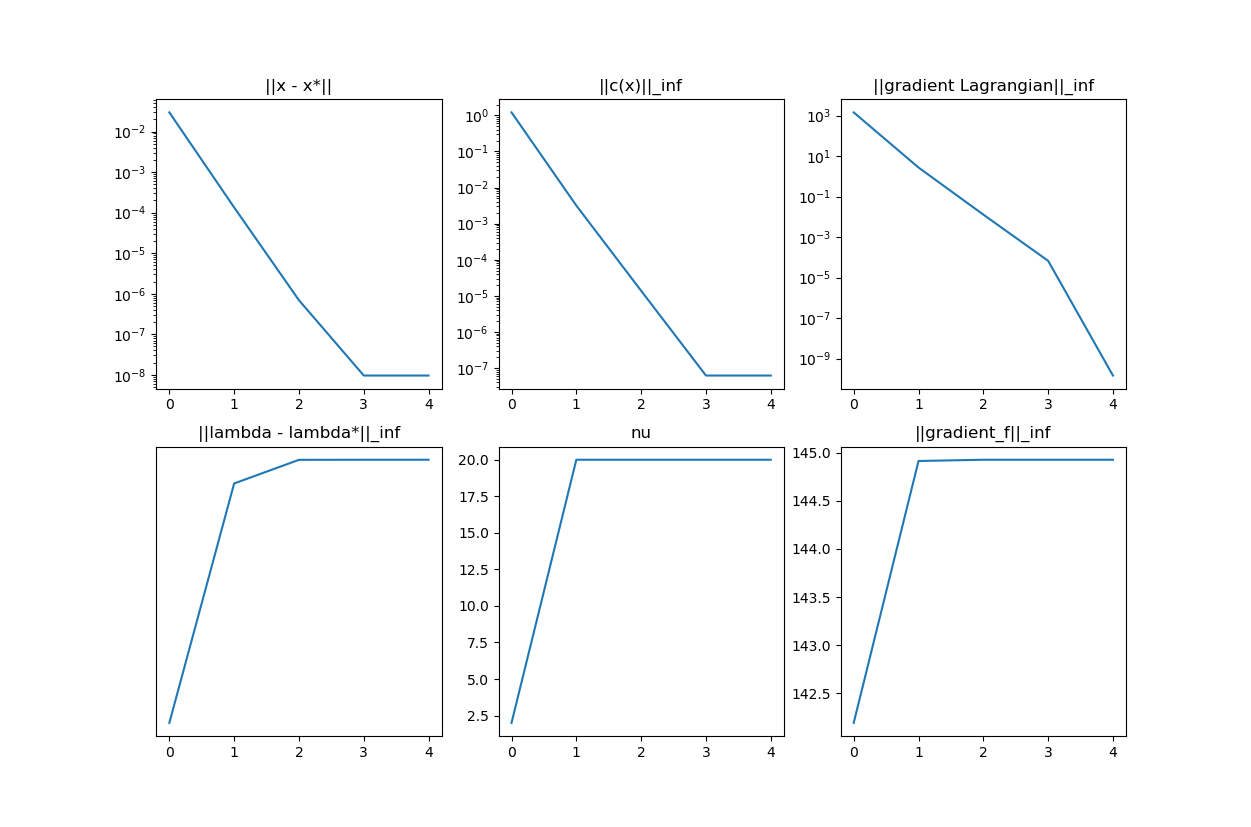
\includegraphics[scale=0.5]{classical3}

\section*{Reminder of Differential calculus}

\begin{theo}[Second order differential of composition of functions]

\begin{multline*}
    D^2(f \circ g)(x)(h_1)(h_2) = \\ Df(g(x))\big(D^2g(x)(h_1)(h_2)\big) + D^2f(g(x))\big(Dg(x)(h_1)\big)\big(Dg(x)(h_2)\big)
\end{multline*}

\end{theo}
\begin{proof}
By the lemma below.
\end{proof}

\medskip
For $f: X \to L(V,W), \ g: X \to L(U, V)$
\begin{defi}[generalized product of functions]
\[
(f \cdot g) (x) := f(x) \circ g(x) 
\]
\end{defi}

\begin{lem}
\[
D(f\cdot g)(x)(h) = f(x) \circ Dg(x)(h) + Df(x)(h) \circ g(x) 
\]
\end{lem}

\begin{remark}
Books remain silent about this theorem. Either not mentioned or in a false expression.
\end{remark}

%\bibliography{report}
%\printbibliography

\end{document}
